\documentclass[10pt,a4paper]{article}
%% Language and font encodings
\usepackage[british]{babel}
\usepackage[utf8]{inputenc}
\usepackage[T1]{fontenc}
%% Sets page size and margins
\usepackage[a4paper,top=2cm,bottom=2cm,left=2.5cm,right=2.5cm,marginparwidth=1.5cm]{geometry}
%% Useful packages
\usepackage{amsmath}
\usepackage{graphicx}
\usepackage[colorlinks=true, allcolors=blue,]{hyperref}
\usepackage{authblk}
\usepackage[backend=biber,style=numeric-comp]{biblatex}
\usepackage{listings}
\usepackage{xcolor}
\usepackage{amsmath} \allowdisplaybreaks% lets align equations break over pages.
\usepackage{amssymb}
\usepackage{caption}
\usepackage{cleveref}
\usepackage{subcaption}
\definecolor{codegreen}{rgb}{0,0.6,0}
\definecolor{codegray}{rgb}{0.5,0.5,0.5}
\definecolor{codepurple}{rgb}{0.58,0,0.82}
\definecolor{backcolour}{rgb}{0.95,0.95,0.92}


% \addbibresource{references.bib}

\lstdefinestyle{mystyle}{
  backgroundcolor=\color{backcolour},
    commentstyle=\color{codegreen},
    keywordstyle=\color{magenta},
    numberstyle=\tiny\color{codegray},
    stringstyle=\color{codepurple},
    basicstyle=\ttfamily\footnotesize,
    breakatwhitespace=false,
    breaklines=true,
    captionpos=b,
    keepspaces=true,
    numbers=left,
    numbersep=5pt,
    showspaces=false,
    showstringspaces=false,
    showtabs=false,
    tabsize=2
}
\lstset{style=mystyle}

\graphicspath{{./img/}}

%% Title
\title{
  {\Huge Simulation and Performance Evaluation}\\
  \huge Homework 4\\
}

\author{Blascovich Alessio and Di Noia Matteo}

\begin{document}

\maketitle

\section*{Simulation Set-Up}

In the simulation the times, between two consecutive packet arrivals and the service time for a packet, follow an exponential distribution of parameters \(\lambda\) and \(\mu\) respectively.

The simulation consists in a FIFO queue of packets arrived that need to be served by a processor.

% explain the computation of the variance and state the confidence interval level used
For measuring it we computed the mean estimators of the parameters searched and also their variance which was used to compute a confidence interval (CI) with 95\% confidence level.

\section*{Exercise 1}

We can start by showing how a simulation evolves over time with particular focus on the number of packets in the queue and in processing. Assuming a single packet can be processed at a time.

\begin{center}
  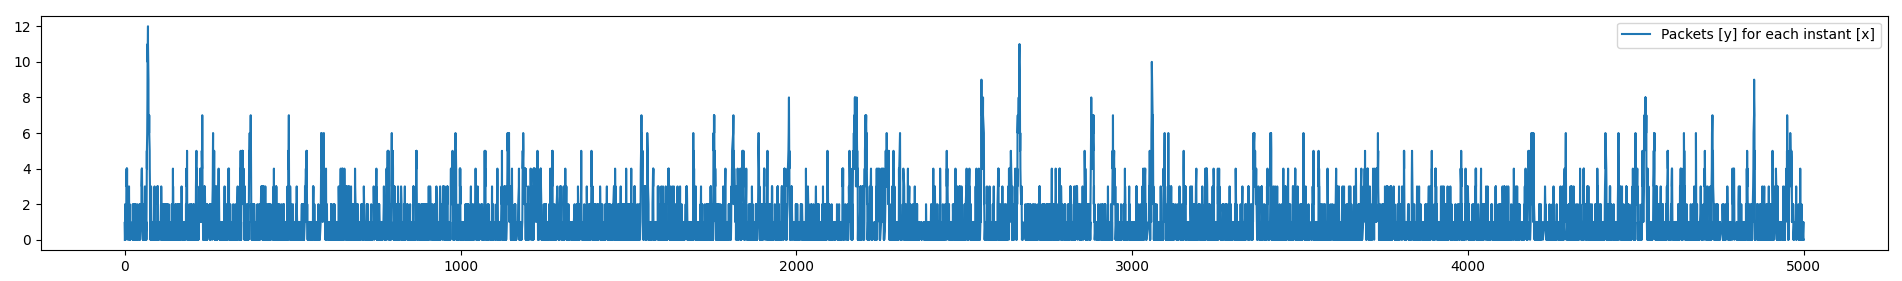
\includegraphics[width=\textwidth]{whole-simulation.png}
  \captionof{figure}{Number of packets in the queue throughout a simulation with \(\lambda = 1\) and \(\mu = 2\)}
\end{center}

% put exponential and log graph about the quantity of packets over time
We started by plotting the distribution of number of packets for each time instant. This distribution is given by summing the enqueued packets plus one if a packet is being processed. We found out, as expected, that such distribution is exponential. We can be sure of this by plotting it with logarithm scale, compute the line that best fit the new data and compute the fit of such a line. The resulting line is in the case \Cref{fig:time-with-fixed-packet-n} is \(-0.385 \cdot x +  9.710\). This line is a good fit for our distribution, since the \(R^2\) test of fitness for our line returns 0.992 (where 1 is a perfect fit).
From this we could easily construct, by elevating the line function to the power of \(e\), the best exponential fit.
\begin{center}
	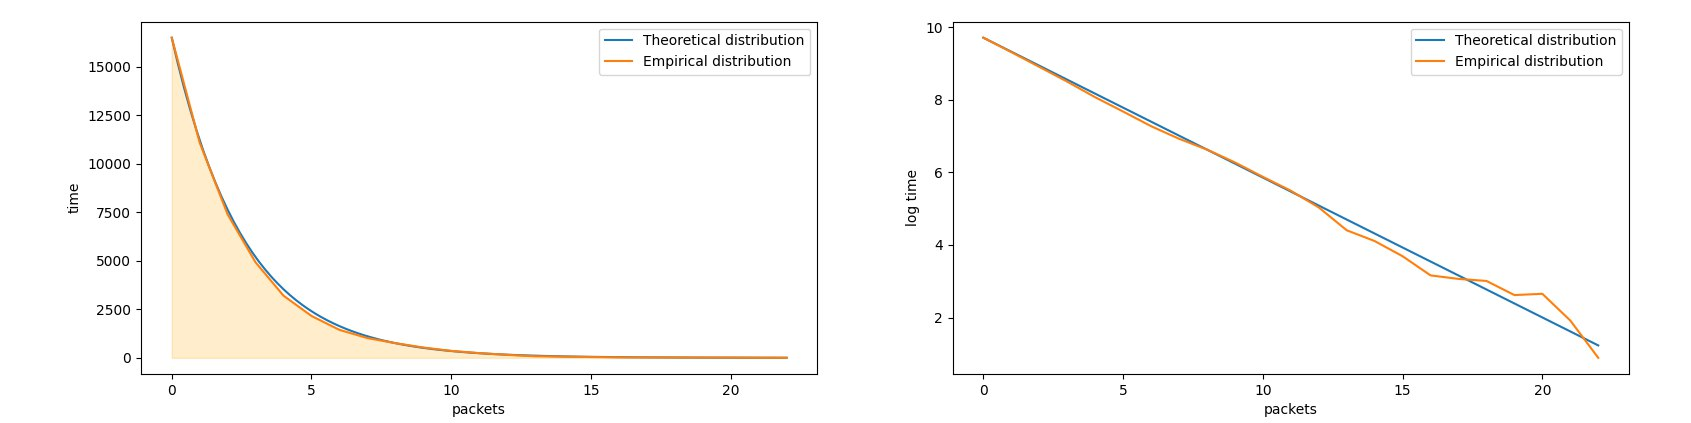
\includegraphics[width=\textwidth]{img/time-with-fixed-packet-n.png}
	\captionof{figure}{Distribution of packets per time instant, \(\lambda = 1\) and \(\mu = 1.5\)}
	\label{fig:time-with-fixed-packet-n}
\end{center}


\subsection*{Independent Replication}

\begin{center}
	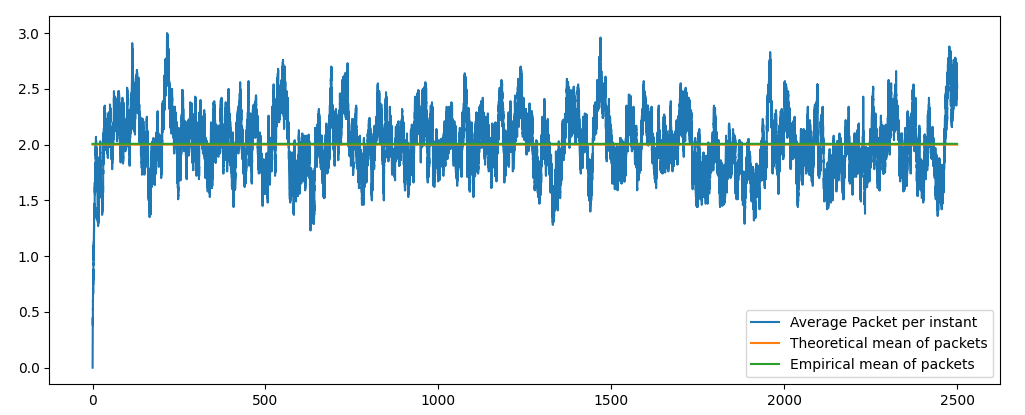
\includegraphics[width=0.7\textwidth]{independent-replication-with-bias.png}
	\captionof{figure}{Independent replication with initialisation bias, \(\lambda = 1\) and \(\mu = 1.5\)}
	\label{fig:independent-replication-with-bias}
\end{center}

We started using ``Independent Replication'' as method to gather information about the number of packets in the queue given a time instant. This method has many advantages, especially for finite state simulations, but can be used as well for steady state analysis; although you have to take into consideration some possible issues such as initialisation problem, introducing periodicity and some others. As such we used this method for qualitative analysis and to compare the other methods used.


Using ``Independent Replication'' we had to take into consideration the initialisation bias that is clearly visible in the left hand-side of~\Cref{fig:independent-replication-with-bias}. This bias is caused by all simulations starting with an empty queue, i.e. 0 packets, at the same time namely instant 0. To overcome this problem there are many solutions:
\begin{itemize}
\item Starting the simulation at a different initial time, starting gathering data after all the simulation have started;
\item Running the simulation for a longer period of time;
\item Discard the first data, using some criteria.
\end{itemize}

We chose the latter method by discarding the first \emph{n} time instants from each simulation, with \emph{n} defined as a multiple of the average number of packets in the system in stationary conditions. However this technique works only in non-divergent simulations (\(\lambda\geq\mu\)) as in those cases the average tends to infinite, this is the case for all the other methods that use the average number of packets in the system. In those cases it is possible to only compute a function describing the climb rate of the average number of packets.

\begin{center}
  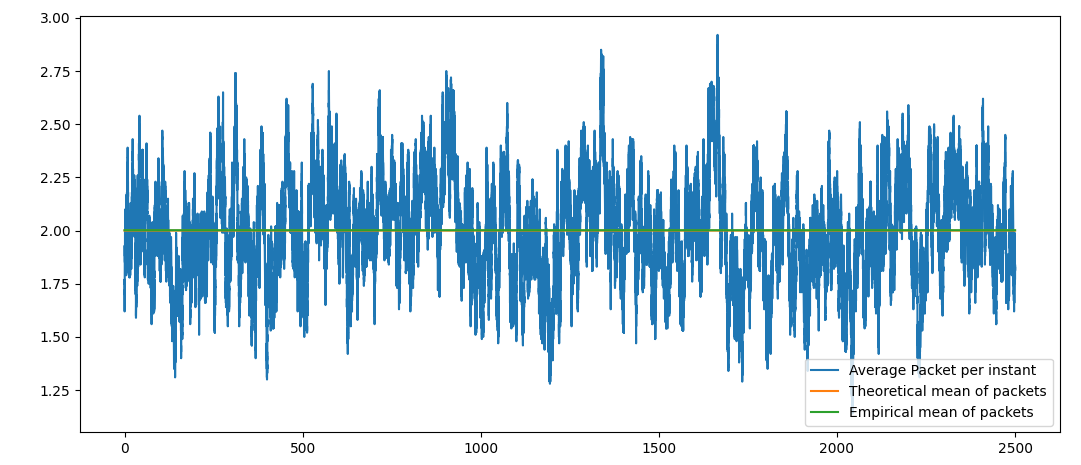
\includegraphics[width=0.7\textwidth]{independent-replication-without-bias.png}
  \captionof{figure}{Independent replication without initialisation bias, \(\lambda = 1\) and \(\mu = 1.5\)}
  \label{fig:independent-replication-without-bias}
\end{center}

Discarding the first \emph{n} time instant we passed from an average of \(2.007 \pm 0.0438\)(\Cref{fig:independent-replication-with-bias}) to an average of \(2.002 \pm 0.0405\)(\Cref{fig:independent-replication-without-bias}), with a theoretical value of 2. While the graph in~\Cref{fig:independent-replication-without-bias} is more representative of the real average over time of a stationary conditions, the obtained average and relative CI do not get much better since the length of the simulation, already partially overwhelm the initialisation bias.

\subsection*{Overlapping Batch Means}

Then we used ``Overlapping Batch Means'' as method to estimate data mean and variance. Since for this method only one simulation is involved, we decided to augment the length of it. The new length used was \(\mathit{number~of~simulations}\times\mathit{length~of~single~simulation}\) used for the ``Independent Replication'' method.

To use this method we must have:
\begin{itemize}
\item Normally distributed batch data;
\item IID data.
\end{itemize}

The second condition is easily verified since every time interval is generated independently and with the same parameters. To satisfy both conditions we picked as batch size \(\mathit{simulation~length} / 1000\) and as number of batch \(10000\) so that they are also overlapping for sure.

Given the theoretical mean is still 2, since we used the same parameters. Some of the empirical means obtained are \( 1.987 \pm 0.0058\), \(2.006 \pm 0.0059\), \(2.010 \pm 0.0062\) and \(1.997 \pm 0.0058\). The CIs obtained are strongly under-estimate for the confidence level of 95\%, to reach the confidence level the obtained CIs should be doubled in size. This problem is due to the fact that this method tends to under-estimate the variance and the fact that probably we are not completely fulfilling the prerequisites of this method.

To conclude, we expected to achieve better results using this method; however the ``Independent Replication'' method gave better results (especially confidence intervals) and was easier to work with.

\subsection*{Varying parameters}

%TODO Quote the usage of rho insert bottom left ex1 graph with rho = 2, 1, 0.90, 0.1
We analysed the convergence of the system with different values of \(\rho\), which is defined as \(\frac \lambda \mu\). We expect that for \(\rho \ge 1\) the data would have been divergent, value closer to 1 to take accumulate larger queue with higher probability while value closer to 0 to tend to be have smaller queue and dispatch them quickly.

\begin{figure}[h]
  \begin{subfigure}[t]{.45\textwidth}
    \centering
    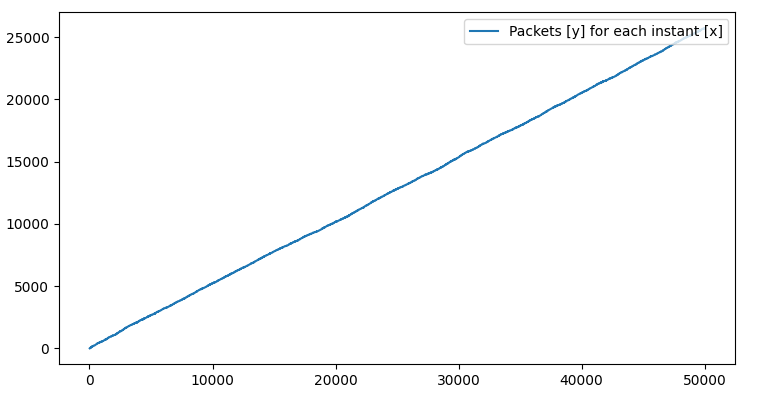
\includegraphics[width=\linewidth]{img/pho2}
    \caption{\(\rho = 2\)}
    \label{fig:rho2}
  \end{subfigure}
  \hfill
  \begin{subfigure}[t]{.45\textwidth}
    \centering
	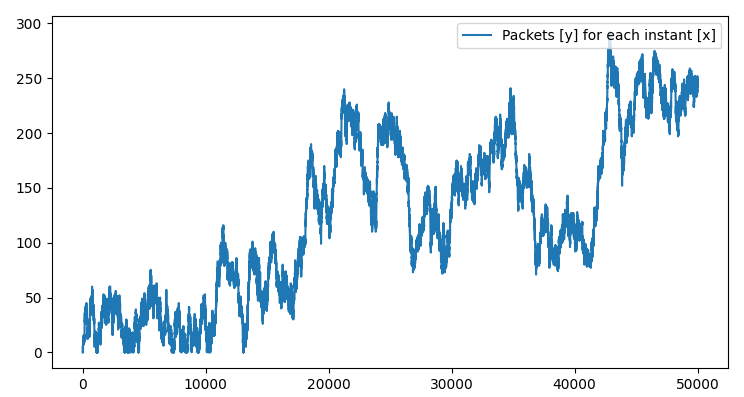
\includegraphics[width=\linewidth]{img/rho1}
    \caption{\(\rho = 1\)}
	\label{fig:rho1}
  \end{subfigure}
  \medskip
  \begin{subfigure}[t]{.45\textwidth}
    \centering
	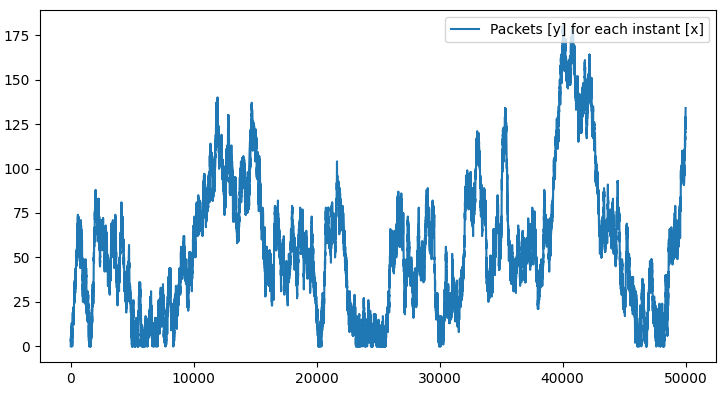
\includegraphics[width=\linewidth]{img/rho0.99}
    \caption{\(\rho = 0.99\)}
	\label{fig:rho099}
  \end{subfigure}
  \hfill
  \begin{subfigure}[t]{.45\textwidth}
    \centering
	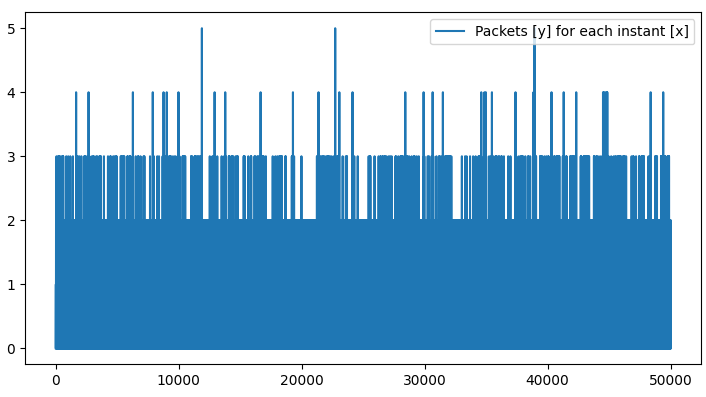
\includegraphics[width=\linewidth]{img/rho0.1}
    \caption{\(\rho = 0.1\)}
	\label{fig:rho010}
  \end{subfigure}
  \caption{Packets per instants with different \(\rho\)}
\end{figure}
  

In \Cref{fig:rho2,fig:rho1} the main difference between the two is that while the first graph has a faster and a lesser irregular rate of climb; the other climbs slower and more irregularly. In \Cref{fig:rho099,fig:rho010}  we see that the first example almost resemble the divergent case, creating large queue. Instead the second, having a much smaller \(\rho\), can dispatch the packets blazingly fast, emptying the queue very often.

\section*{Exercise 2}

For this exercises we used \(\rho = \frac{2}{7}\) so that the the theoretical average traversal time for any packet is 0.4.

To compute the variance of the mean two methods where employed:
\begin{itemize}
\item A naive method, the variance of all the measurements;
\item ``Post-stratification'', defining a stratum as the number of packets in the queue in when another packet arrives.
\end{itemize}

\subsection*{Pseudo-Code}

\begin{lstlisting}[language=python,caption={Post-stratification pseudo-code},captionpos=b,label={lst:post-stratififcation}]
lenght = max(dep_queue_waiting) + 1
stratified = [[] for _ in range(lenght)]

for inqueue, elapsed in zip(dep_queue_waiting, dep_elapsed):
    stratified[inqueue].append(elapsed)

strati_mean = []
strati_var = []
strati_pi = []
for stratum in stratified:
    strati_mean.append(np.average(stratum))
    strati_var.append(stratum))
    strati_pi.append(len(stratum) / len(dep_queue_waiting))

post_stratified_avg = 
    np.average(strati_mean, weights=strati_pi)

post_stratified_var =
    np.average(strati_var, weights=strati_pi) / len(stratified)
\end{lstlisting}

In \Cref{lst:post-stratififcation} we only describe ``Post-stratification'' since the naive code is trivial.

\subsection*{Analysis}

To compare the alternatives, we used ``Comparison of alternatives''. In this simulation  data are correlated,therefore we used ``Correlated case''. For each simulation we computed:

\begin{equation*}
  \mathit{d}_i = \mathit{post\ stratum\ var}_i - \mathit{naif\ var}_i
\end{equation*}

We then computed the average of the differences, its variance and CI. In \Cref{fig:post-stratification} are shown the difference (blue), average (orange), and lower/upper bounds (green and red respectively).

\begin{center}
  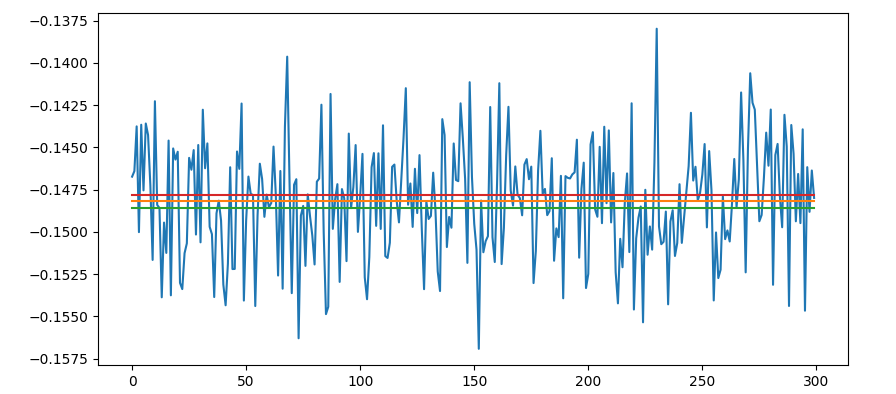
\includegraphics[width=0.8\textwidth]{post-stratification.png}
  \captionof{figure}{Difference of the two methods, \(\rho = \frac{2}{7}\)}
  \label{fig:post-stratification}
\end{center}

In \Cref{fig:post-stratification} it is possible to see all the values, and 95\% Confidence level of the mean are negative. As such we can conclude with such confidence level that the second method (``Post-stratification'') has a lower variance that the naive method.

In particular the average of the variance of the second method is 10 times lower than the average of the first method.

\end{document}
